\documentclass{article}
\usepackage{graphicx}

\title{The Story of 24 Point}
\author{Owen Xuan}

\begin{document}

\maketitle
Start with four cards, face up. Glance at their numbers: $7, 6, 12, 4$. The aim of the game is to manipulate these four numbers into equalling twenty-four, by using multiplication, division, addition, subtraction, and parenthesis. Aha! You find a solution:  $12 \times 6 / (7-4)$ equals twenty-four. Among other names, this card game is named 24 point. Standing on a deceptively straightforward foundation, 24 point is both malleable and lively. 

My first experience with 24 point came when I was 7, likely playing at our dinner table. We would split the deck into halves, then have each player flip two cards over and arrange them in a square. Thus ensued a state of full concentration: each round ended in either mutual shaking of heads and a redraw, or an excited table slap, which signaled a player had found a solution. Soon, I found myself bringing a deck of Bicycle playing cards on the bus, solving puzzles against an imaginary opponent. A distinctive quality of 24 point was that it could easily be played with a single person, and was portable, unlike solitaire. 

\begin{center}
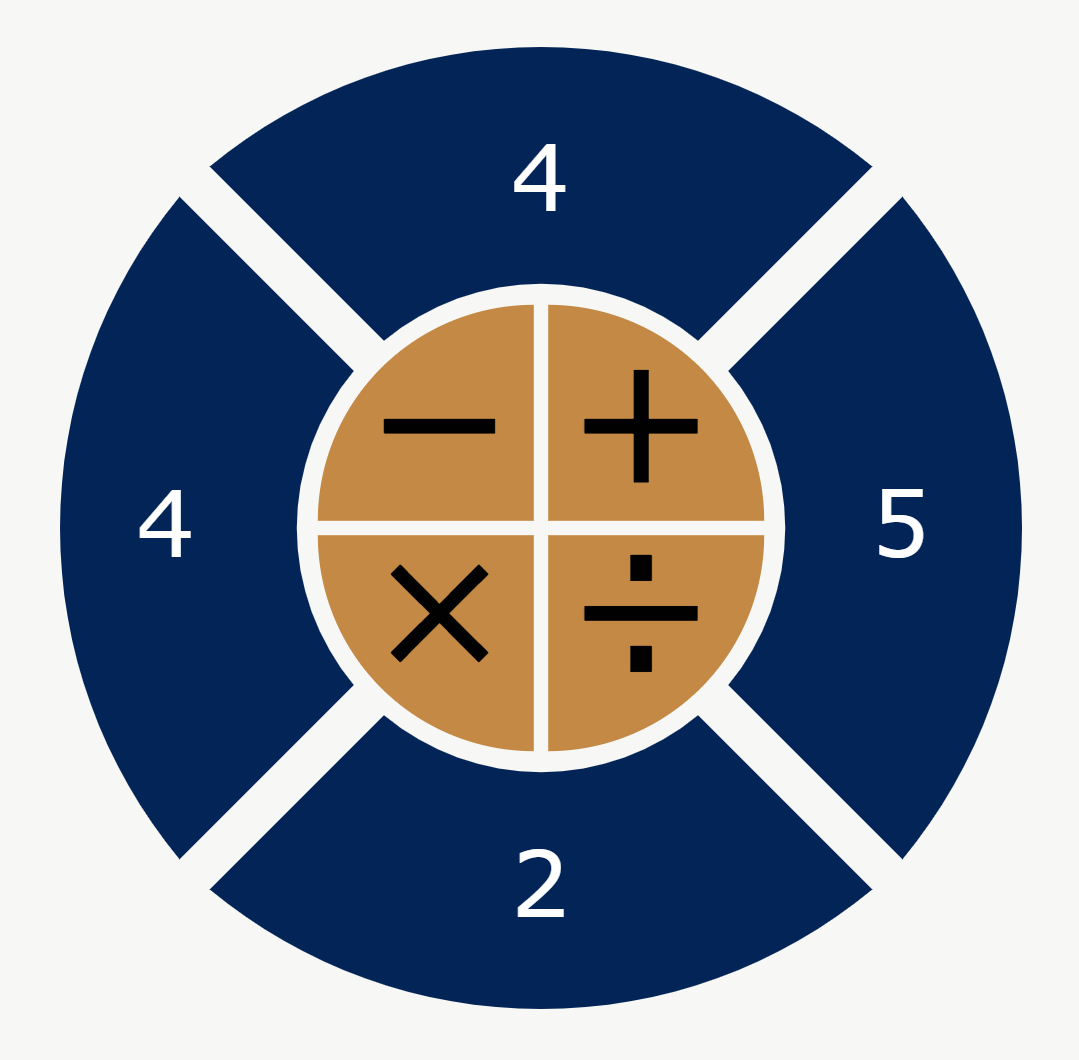
\includegraphics[scale=0.25]{images/24.png}
\end{center}

There’s a certain beauty to the complexity arising from the simple framework. Some arrangements of four cards are clear at a glance, whereas others, notably $[3 3 8 8]*$, look easy but require some thought. If we allow order and parenthesis to matter, even the combination $[1 2 3 4]$ has 194 solutions. Over time, certain puzzle-solving rules of thumb emerge. One quick technique is to build factors of 24, most commonly 3, 8 and 4, 6. Another strategy is to go a bit over 24, then subtract a card to return to the desired number, such as in the case $[3 3 3 3]$.

As one might expect, there are many arrangements of cards which are impossible to solve. With our current rules, $[1 1 1 1]$ is impossible (easy to verify), and so is $[3 3 5 11]$ (harder to verify). A full database of solvable and unsolvable combinations can be found here. Interestingly, around $25\%$ of combinations are unsolvable with our current available operators $(+ - * /)$ but if we introduce factorials, this number drops twenty-five fold to just below $1\%$. 

Perhaps the most valuable quality of the game is its adaptability. Since the main theme of the game is to create one number out of four, it can be modified without losing its nature. Frequently, players will allow new operators to boost the probability of getting a solvable set of cards, such as allowing exponentiation, square roots and logarithms. Factorials and permutations are also sometimes added, although some argue that it makes the game too easy (simply getting to 4, then using the factorial operator gets to 24). Other semi-common changes include changing the target number or changing the amount of cards used.

If we wish to venture beyond these standard variations, 24 point can be engineered to become more challenging, or cover concepts from more diverse fields of mathematics. To do this, we can increase the difficulty in two steps: removing “simple” operators and adding “complex” ones. Instead of using addition $(f(x,y) = x+y)$, what if we let $f(x,y) = 3x+y$? Or let an operator return the sum of the digits of the product of the two inputs? Or, going on a wild limb, creating an operator which takes in n cards, calculates the derivative of the polynomial $P(x) = x(\sum_{i=1}^n (a_i \cdot x^i))$, and returns the sum of the resulting coefficients? Once one starts tinkering with alterations, the flexibility of the game becomes obvious.

For educators, 24 point is an ideal game to both stimulate the brain and provide breaks from lectures. In addition to its flexibility, 24 point can provide a degree of competitive spirit (while still retaining some element of chance, for weaker students), or alternatively can be played in teams. The game is ripe with patterns, meaning players will likely feel a sense of progress as they begin to recognize more and more patterns within the random combinations of cards. Moreover, unlike the majority of “math games” within schools – even with discounting coolmathgames – 24 point builds arithmetic skills and critical thinking. In short, 24 point has the perfect build for a math game: short and sweet, helpful, flexible, satisfying.
\end{document}